\documentclass[a4paper]{article}
\usepackage[spanish]{babel}
\usepackage[utf8]{inputenc}
\usepackage{charter}   % tipografia
\usepackage{graphicx}
%\usepackage{makeidx}
\usepackage{paralist} %itemize inline

%\usepackage{float}
%\usepackage{amsmath, amsthm, amssymb}
%\usepackage{amsfonts}
%\usepackage{sectsty}
%\usepackage{charter}
%\usepackage{wrapfig}
%\usepackage{listings}
%\lstset{language=C}


\usepackage{color} % para snipets de codigo coloreados
\usepackage{fancybox}  % para el sbox de los snipets de codigo

\definecolor{litegrey}{gray}{0.94}

% \newenvironment{sidebar}{%
% 	\begin{Sbox}\begin{minipage}{.85\textwidth}}%
% 	{\end{minipage}\end{Sbox}%
% 		\begin{center}\setlength{\fboxsep}{6pt}%
% 		\shadowbox{\TheSbox}\end{center}}
% \newenvironment{warning}{%
% 	\begin{Sbox}\begin{minipage}{.85\textwidth}\sffamily\lite\small\RaggedRight}%
% 	{\end{minipage}\end{Sbox}%
% 		\begin{center}\setlength{\fboxsep}{6pt}%
% 		\colorbox{litegrey}{\TheSbox}\end{center}}

\newenvironment{codesnippet}{%
	\begin{Sbox}\begin{minipage}{\textwidth}\sffamily\small}%
	{\end{minipage}\end{Sbox}%
		\begin{center}%
		\vspace{-0.4cm}\colorbox{litegrey}{\TheSbox}\end{center}\vspace{0.3cm}}



\usepackage{fancyhdr}
\pagestyle{fancy}

%\renewcommand{\chaptermark}[1]{\markboth{#1}{}}
\renewcommand{\sectionmark}[1]{\markright{\thesection\ - #1}}

\fancyhf{}

\fancyhead[LO]{Sección \rightmark} % \thesection\ 
\fancyfoot[LO]{\small{Alejandro Mignanelli, Franco Negri, Federico Suárez}}
\fancyfoot[RO]{\thepage}
\renewcommand{\headrulewidth}{0.5pt}
\renewcommand{\footrulewidth}{0.5pt}
\setlength{\hoffset}{-0.8in}
\setlength{\textwidth}{16cm}
%\setlength{\hoffset}{-1.1cm}
%\setlength{\textwidth}{16cm}
\setlength{\headsep}{0.5cm}
\setlength{\textheight}{25cm}
\setlength{\voffset}{-0.7in}
\setlength{\headwidth}{\textwidth}
\setlength{\headheight}{13.1pt}

\renewcommand{\baselinestretch}{1.1}  % line spacing


% \setcounter{secnumdepth}{2}
\usepackage{underscore}
\usepackage{caratula}
\usepackage{url}


% ******************************************************** %
%              TEMPLATE DE INFORME ORGA2 v0.1              %
% ******************************************************** %
% ******************************************************** %
%                                                          %
% ALGUNOS PAQUETES REQUERIDOS (EN UBUNTU):                 %
% ========================================
%                                                          %
% texlive-latex-base                                       %
% texlive-latex-recommended                                %
% texlive-fonts-recommended                                %
% texlive-latex-extra?                                     %
% texlive-lang-spanish (en ubuntu 13.10)                   %
% ******************************************************** %



\begin{document}


\thispagestyle{empty}
\materia{Organización del Computador II}
\submateria{Segundo Cuatrimestre de 2014}
\titulo{Trabajo Práctico III}
\subtitulo{El Kernel contraataca}
\integrante{Alejandro Mignanelli}{609/11}{minga_titere@hotmail.com}
\integrante{Franco Negri}{893/13}{franconegri2004@hotmail.com}
\integrante{Federico Suárez}{610/11}{elgeniofederico@gmail.com}

\maketitle
\newpage

\thispagestyle{empty}
\vfill
\begin{abstract}
En el presente trabajo se describe el desarrollo del Kernel para una arquitectura intel de 32-bits, así como el manejo de paginación, manejo de tareas, interrupciones y todo lo referente al manejo de un pequeño sistema operativo.

\end{abstract}

\thispagestyle{empty}
\vspace{3cm}
\tableofcontents
\newpage

%\normalsize
\newpage

\section{Objetivos generales}

El objetivo de este trabajo práctico es, partiendo de un procesador intel de 32-bits, generar un kernel capaz de gestionar memoria entre diferentes tareas, correrlas de manera concurrente, y resolver las diferentes problemáticas que puedan surgir al momento de ejecución.

Para ello utilizaremos las diversas herramientas que intel pone a nuestra disposición en modo protegido: Usaremos segmentación y paginación para controlar el privilegio con el que las tareas se ejecutarán, además de limitar lo que las tareas puedan 'ver' con un mapeo parcial de la memoria.
Utilizaremos interrupciones del procesador que permitirán, tanto reaccionar de manera apropiada cuando se produzca un error en tiempo de ejecución, obtener input del teclado y gestionar un task manager que nos permita ejecutar tareas de manera concurrente.

En el presente informe, se detallará de manera más elaborada todo lo hecho para lograr el objetivo del trabajo práctico, así como cualquier decisión que se haya tomado en el código a tales fines. Para su mejor entendimiento, este informe se dividirá en ejercicios, que son pequeñas partes del trabajo, y todos juntos conforman al trabajo práctico en sí. 

\section{Ejercicio 1: GDT Basica}
En este primer ejercicio, decidimos completar las primeras $7$ posiciones de la gdt en un estado claramente inválido para que, en caso de usarlos erróneamente en algún momento, el error fuera visible. Luego, pusimos $4$ segmentos, dos para código de nivel 0 y 3, y dos para datos de nivel 0 y 3. Para un mayor entendimiento del código, se han usado defines, con nombres declarativos(por ejemplo, el segmento destinado a código de nivel $0$, se llama GDT_IDX_CDE_LVL_0). Estos segmentos direccionan los primeros 623 MB de memoria. También se ha declarado un segmento que describe el area de la pantalla en memoria que puede ser utilizado sólo por el kernel. Esto se utilizará en principio para escribir en el buffer de memoria, pero más avanzado el trabajo, será necesario mantener muchas estructuras de datos que deberán ser impresas por pantalla, por lo tanto se abandonará este método y se pasará a un código en C, más limpio y fácil de mantener. Dado que la convención C nos pide que todos los segmentos de datos apunten al mismo segmento, este segmento terminará quedando en desuso y se utilizará para escribir en pantalla tan sólo el segmento de datos de nivel 0. Después, para pasar a modo protegido, deshabilitamos las interrupciones, habilitamos el $A20$, cargamos la GDT, seteamos el bit PE del registro CR0 en $1$ para habilitar modo protegido, y luego hacemos un jump far a un segmento válido para pasar efectivamente a modo protegido. Una vez hecho el pasaje, seteamos todos los segmentos para que apunten al mismo descriptor de segmento (pedido por la convención c) y seteamos la base y puntero de la pila del kernel en la posición $0x27000$. Finalmente inicializamos en pantalla la interfaz gráfica que tendrá el juego, para lo cual utilizamos el segmento anteriormente mencionado.

La antigua implementación para actualizar pantalla y un rudimentario print(char *) que todavía se utiliza en los primeros pasos de inicialización, pueden verse en $screen.asm$.

%\input{GDT/gdt.tex}

\section{Ejercicio 2: IDT Basica} 
%\input{Interrupciones/int.tex}

En este ejercicio inicializamos la IDT, es decir, completamos las entradas necesarias para asociar diferentes rutinas a todas las excepciones del procesador. En principio, cada una de estas rutinas mostrará por pantalla qué tipo de problema se produjo e interrumpirá la ejecución. Luego de inicializada la IDT, deberemos cargarla desde el kernel. Posteriormente se modicarán estas rutinas para que en caso de que sea una tarea de nivel 3 se resuelva el problema y se desaloje a la tarea que lo produjo.
En caso de producirse un error de kernel, se mostrará a qué tipo pertenece y en caso de tener, su code error.

\section{Ejercicio 3: Paginación Basica}
%\input{MMU/mmu.tex}

Inicializamos el directorio de páginas del kernel y las tablas de páginas necesarias para mapear las direcciones 0x00000000 a 0x003FFFFF usando identity mapping y para ello usamos un pequeño código en assembler que puede verse en $paging.asm$. En principio esta función era suficiente para el simple mapeo que requeríamos. Más adelante se optará por inicializar los directorios de páginas y tablas de páginas de una manera más clara y limpia utilizando $mmu.c$. El directorio de páginas del kernel se inicializará en la dirección $0x27000$ y las tablas de páginas a partir de la dirección $0x28000$. En este paso, se implementa una función llamada pedirPag, que dada la dirección de una página, la inicializa con todas sus entradas en cero, poniendo exclusivo cuidado en setear en 0 el bit de "presente" en cada caso, de manera que no sea utilizada hasta que se determine una dirección apropiada para la misma. 
Luego de armado el directorio de páginas del kernel, seteamos el CR3 para que apunte al directorio de páginas y seteamos en 1 el bit correspondiente del registro CR0 para habilitar la paginación.

\section{Ejercicio 4: Memory Management Unit}
%\input{Paginacion/pag.tex}

Aquí implementamos la Memory Management Unit dentro de $mmu.c$, para ello, primero la inicializamos seteando una variable "dirGlobal" la cual siempre apuntará a una dirección física libre de memoria que será utilizada para alojar una tabla o directorio de página según corresponda.

Luego construimos una función para inicializar zombies ($mmu\_ inicializar\_ zombie$) que recibe como parámetros el código de la tarea y un arreglo de direcciones físicas(éste contiene como primer elemento a la posición en el mapa donde estamos inicializando el zombie, y en el resto del arreglo las 8 posiciones del mapa contiguas). En esta función creamos un nuevo directorio de páginas y una tabla de páginas para la tarea zombie y vinculamos la tabla de páginas del kernel a la primera entrada del directorio de páginas de la tarea zombie. Después, mapeamos cada dirección del arreglo a partir de la dirección virtual 0x8000000. 
Dado que el area del mapa donde se ejecutarán los zombies no es alcanzable desde el kernel deberemos mapear la dirección física donde se encontrará el zombie en alguna dirección virtual que no utilicemos de manera tal que podamos copiar su código a esta dirección, y una vez copiado el código, desmapearlo.

Para eso, agregamos al directorio de páginas actual una nueva tabla de páginas, mapeamos en ella una dirección que no se use (en este caso se decidió $0xDC4000$), copiamos el código, y por último desligamos dicha tabla del directorio de páginas.

Para todo este proceso se implementarán varias funciones que facilitarán la tarea de mapear y desmapear tablas de páginas a direcciones reales y directorios de páginas a tablas, que más adelante cuando sea necesario remapear zombies, resultarán de suma utilidad. Estas funciones simplemente inicializarán entradas tanto en el directorio de paginas como en la tabla de paginas en estados validos.

\section{Ejercicio 5: Interrupciones De Teclado/Reloj}
%\input{Scheduler/scheduler.tex}

Completamos las entradas necesarias en la IDT para asociar las rutinas correspondientes a las interrupciones del teclado, reloj y la interrupción de sofware 0x66. De momento estas funciones no tendrán mayor utilidad, el teclado sólo mostrará un mensaje por pantalla al presionarse una tecla y el reloj solo actualizará un reloj en la parte inferior derecha de la pantalla, pero estos comportamientos nos permiten poder probar que las interrupciones se realizan correctamente.

De momento la interrupción 0x66 no realizará ninguna acción, se hablará de cómo fue implementada mas adelante en el TP.

Posteriormente se reescribirán dichas rutinas para que, la del reloj sea utilizada para actualizar la pantalla y llamar al scheduler y cambiar a la tarea adecuada en cada tick del reloj, la del teclado se utilice para que las distintas teclas respondan a la función asignada y finalmente la interrupción 0x66 que se utilizará para el movimiento de las tareas zombies.

\section{Ejercicio 6: TSS}

En este ejercicio se implementará principalmente el archivo $tss.c$ el cual se encargará de administrar de buena manera todo lo que tenga que ver con el seteo apropiado de las tss a ser utilizadas.

En principio se crea una entrada vacía que será donde guardemos la tss del kernel en el momento en que este deje de ser de utilidad.

Como segundo paso se setea de manera apropiada las variables de la tarea idle en $inicializarTareaIdle()$.

Luego se implementará una función $cargarTSS\_ zombie()$ que se encargue de inicializar 16 entradas en la gdt que corresponderán a cada uno de los zombies que pueden estar activos en el tablero. Esta función primero setea las entradas de la gdt para que apunten unívocamente a un tss a ser utilizada por un zombie y luego se setea la tss correspondiente también en estado válido para que queden listas para ser utilizadas por una tarea de nivel 3. Lo único que quedará sin setear será el CR3 de todas las tss, eso se determinará en el momento en que $mmu\_ inicializar\_ zombie$ nos dé un CR3 valido.

Además, para simplificar las cosas, se tomará como que las primeras 8 tss son de los zombies del jugador A y las siguientes 8 entradas son del jugador B. De esa manera con tan solo tener el indice de que tss se está corriendo, podremos además determinar a que jugador pertenece.

Más adelante se determinará que es mas facil para la implementación elegida, setear la TSS en el momento en que se crea el zombie, por lo que iniciar una nueva tss se convertirá en una función aparte.

Aquí se puede ver la estructura final de nuestra GDT:

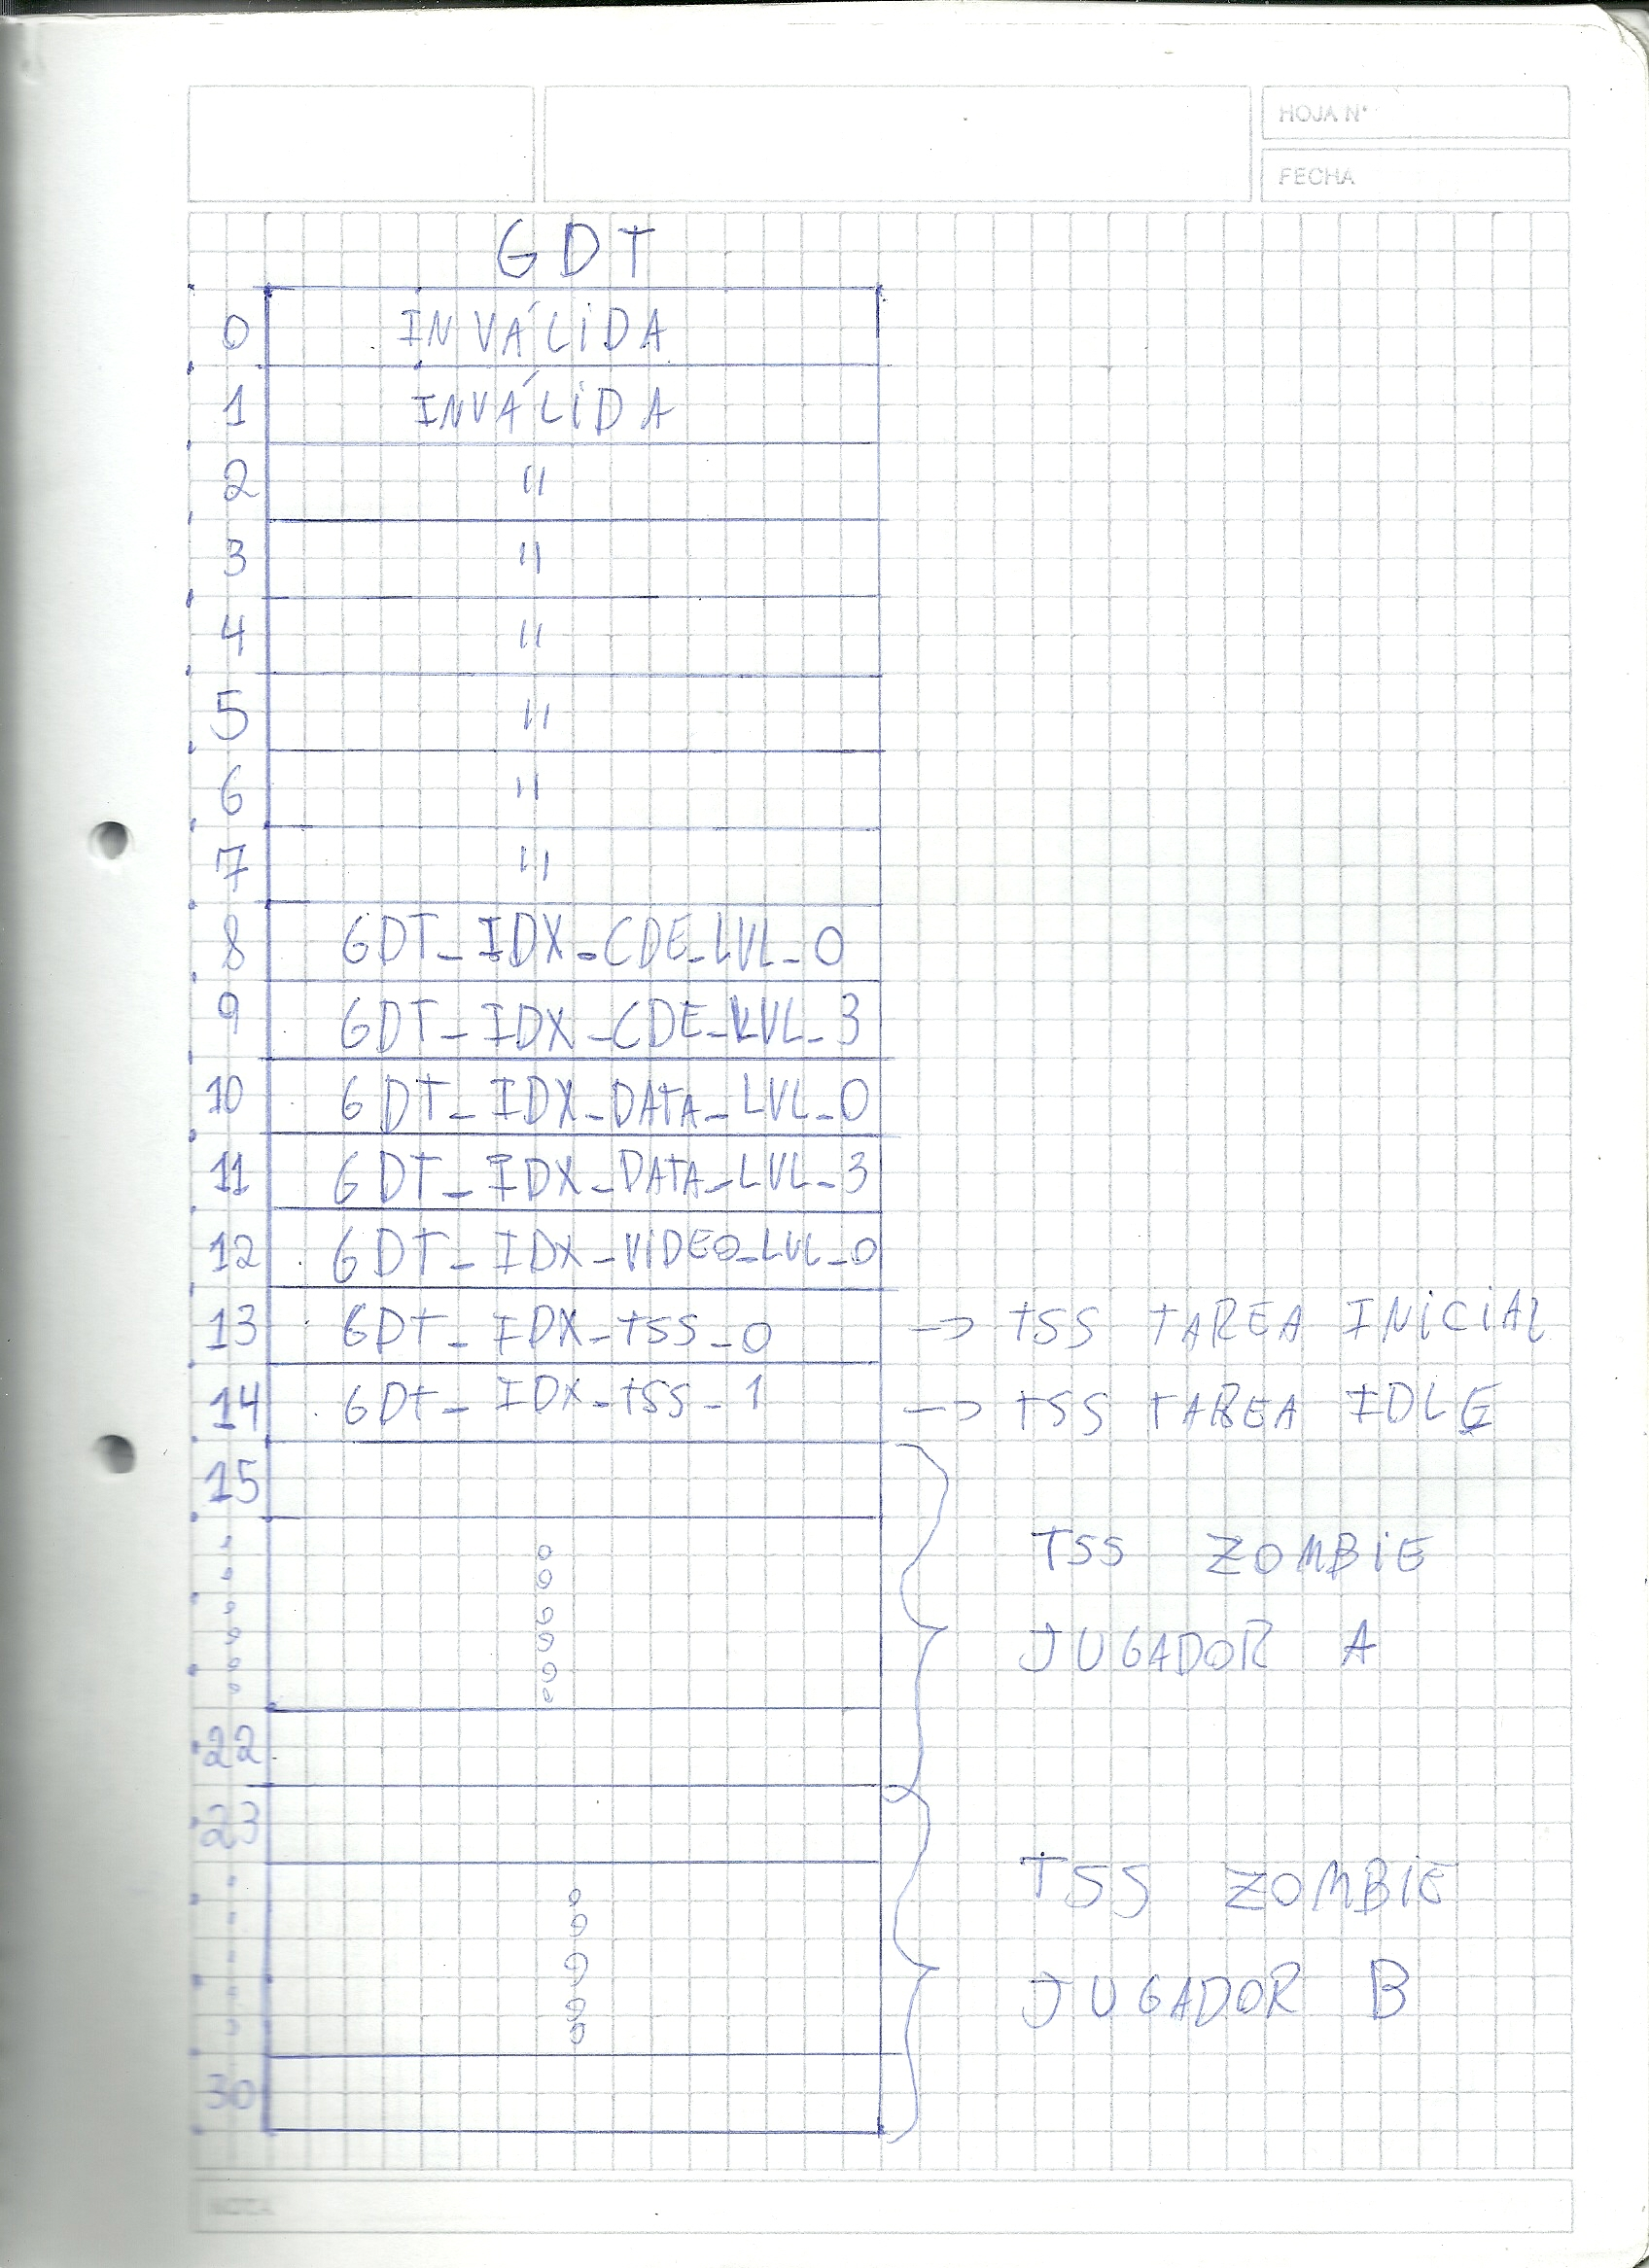
\includegraphics[scale=0.29]{dibujos/dibujo4.jpg}\\

\section{Ejercicio 7: Scheduler}

En este ejercicio se implementa un scheduler simple que a partir de lo devuelto por la función $sched\_ proximo\_ indice()$ (implementada en $sched.c$). Por ahora y dado que no hay otras tareas para correr, este scheduler siempre retornará el valor de la tarea idle, pero más tarde se agregará la lógica para que además alterne entre zombies en el caso en que sea necesario.

En este momento del TP, todavía no contamos con la lógica para saber donde se encuentra un zombie, cómo será la lógica para mapearlo, quién controlará si está o no activo, así que decidimos no seguir de manera estricta la guía proporcionada.

\section{Ejercicio 8: El ensamble Final}

LLegados a este punto tenemos un scheduler, una MMU, 16 TSSs, pero todavía falta implementar toda la lógica del juego propiamente dicho. Lo que se determina es que hace falta una estructura que mantenga las coordenadas en las que el zombie se encuentra, para asi facilitar el mapeo y la escritura en la pantalla. Además hace falta saber a que tipo pertenece cada zombie lanzado, tanto para poder copiar su código de manera efectiva como para poder mostrarlo en pantalla. Hace falta mantener de alguna manera las coordenadas del jugador A y B, los puntajes, la cantidad de zombies disponbiles.

Se determina utilizar $game.c$ para todo ello. Allí se implementará toda la lógica del juego, las posiciones de los jugadores, los puntajes, los zombies activos, las coordenadas de los zombies y los zombes muertos/baba de zombie que pueda haber en el tablero. Dado que $game.c$ posee toda esta información, es lógico pensar que también aquí se maneje la pantalla ya que existe una correspondecia directa entre ambos.

Se crean funciones para que ambos jugadores puedan moverse por la pantalla ($game\_ moverJugador()$), cambiar la clase del próximo zombie que será creado ($game\_ cambiarClase\_ atras()$ y $game\_ cambiarClase\_ adelante()$) y la funcionalidad de lanzar un zombie (ver $game\_ lanzar\_ zombi()$). Todas estas funciones estaran mapeadas por interrupciones de teclado a las teclas correspondientes.

Cabe destacar la funcionalidad de $game\_ lanzar\_ zombi()$ ya que en esta función sucede una parte crítica del juego:

En ella, se buscará primero en una arreglo previamente inicializado (Al cual se llamará $clockZombie$ ), si queda algun zombie "muerto" del jugador que corresponda, o lo que es lo mismo, existe una tarea para el jugador que corresponda que no este siendo utilizada. De ser el caso, se marca en este arreglo que la tarea ha empezado a estar "viva" (principalmente para que esta no pueda ser desplazada por otra tarea), se inicializan las coordenadas X e Y del tablero para el zombie y en base a ella se calculan las direcciones reales que el zombie ocupará.

Una vez que tenemos las direcciones reales del zombie, se procede a inicializarlo llamando a la función $mmu\_ inicializar\_ zombie$ que como ya hemos dicho, mapea estas posiciones donde corresponde. Asi obtenemos el CR3 del zombie.

Ahora limpiamos su tss, que esta unívocamente ligada al arreglo antes mencionado. Aquí es cuando notamos que no es necesario iniciar en $cargarTSS\_ zombie()$ las tss de antemano.

Luego cargamos el CR3 del zombie en su TSS con $mapearCr3Tss()$ y así obtenemos una tss limpia para poder empezar a ejecutar el zombie.

Este es el esquema grafico para ver como funcióna todo el sistema en conjunto:


%\begin{figure}[h!]
%  \begin{center}
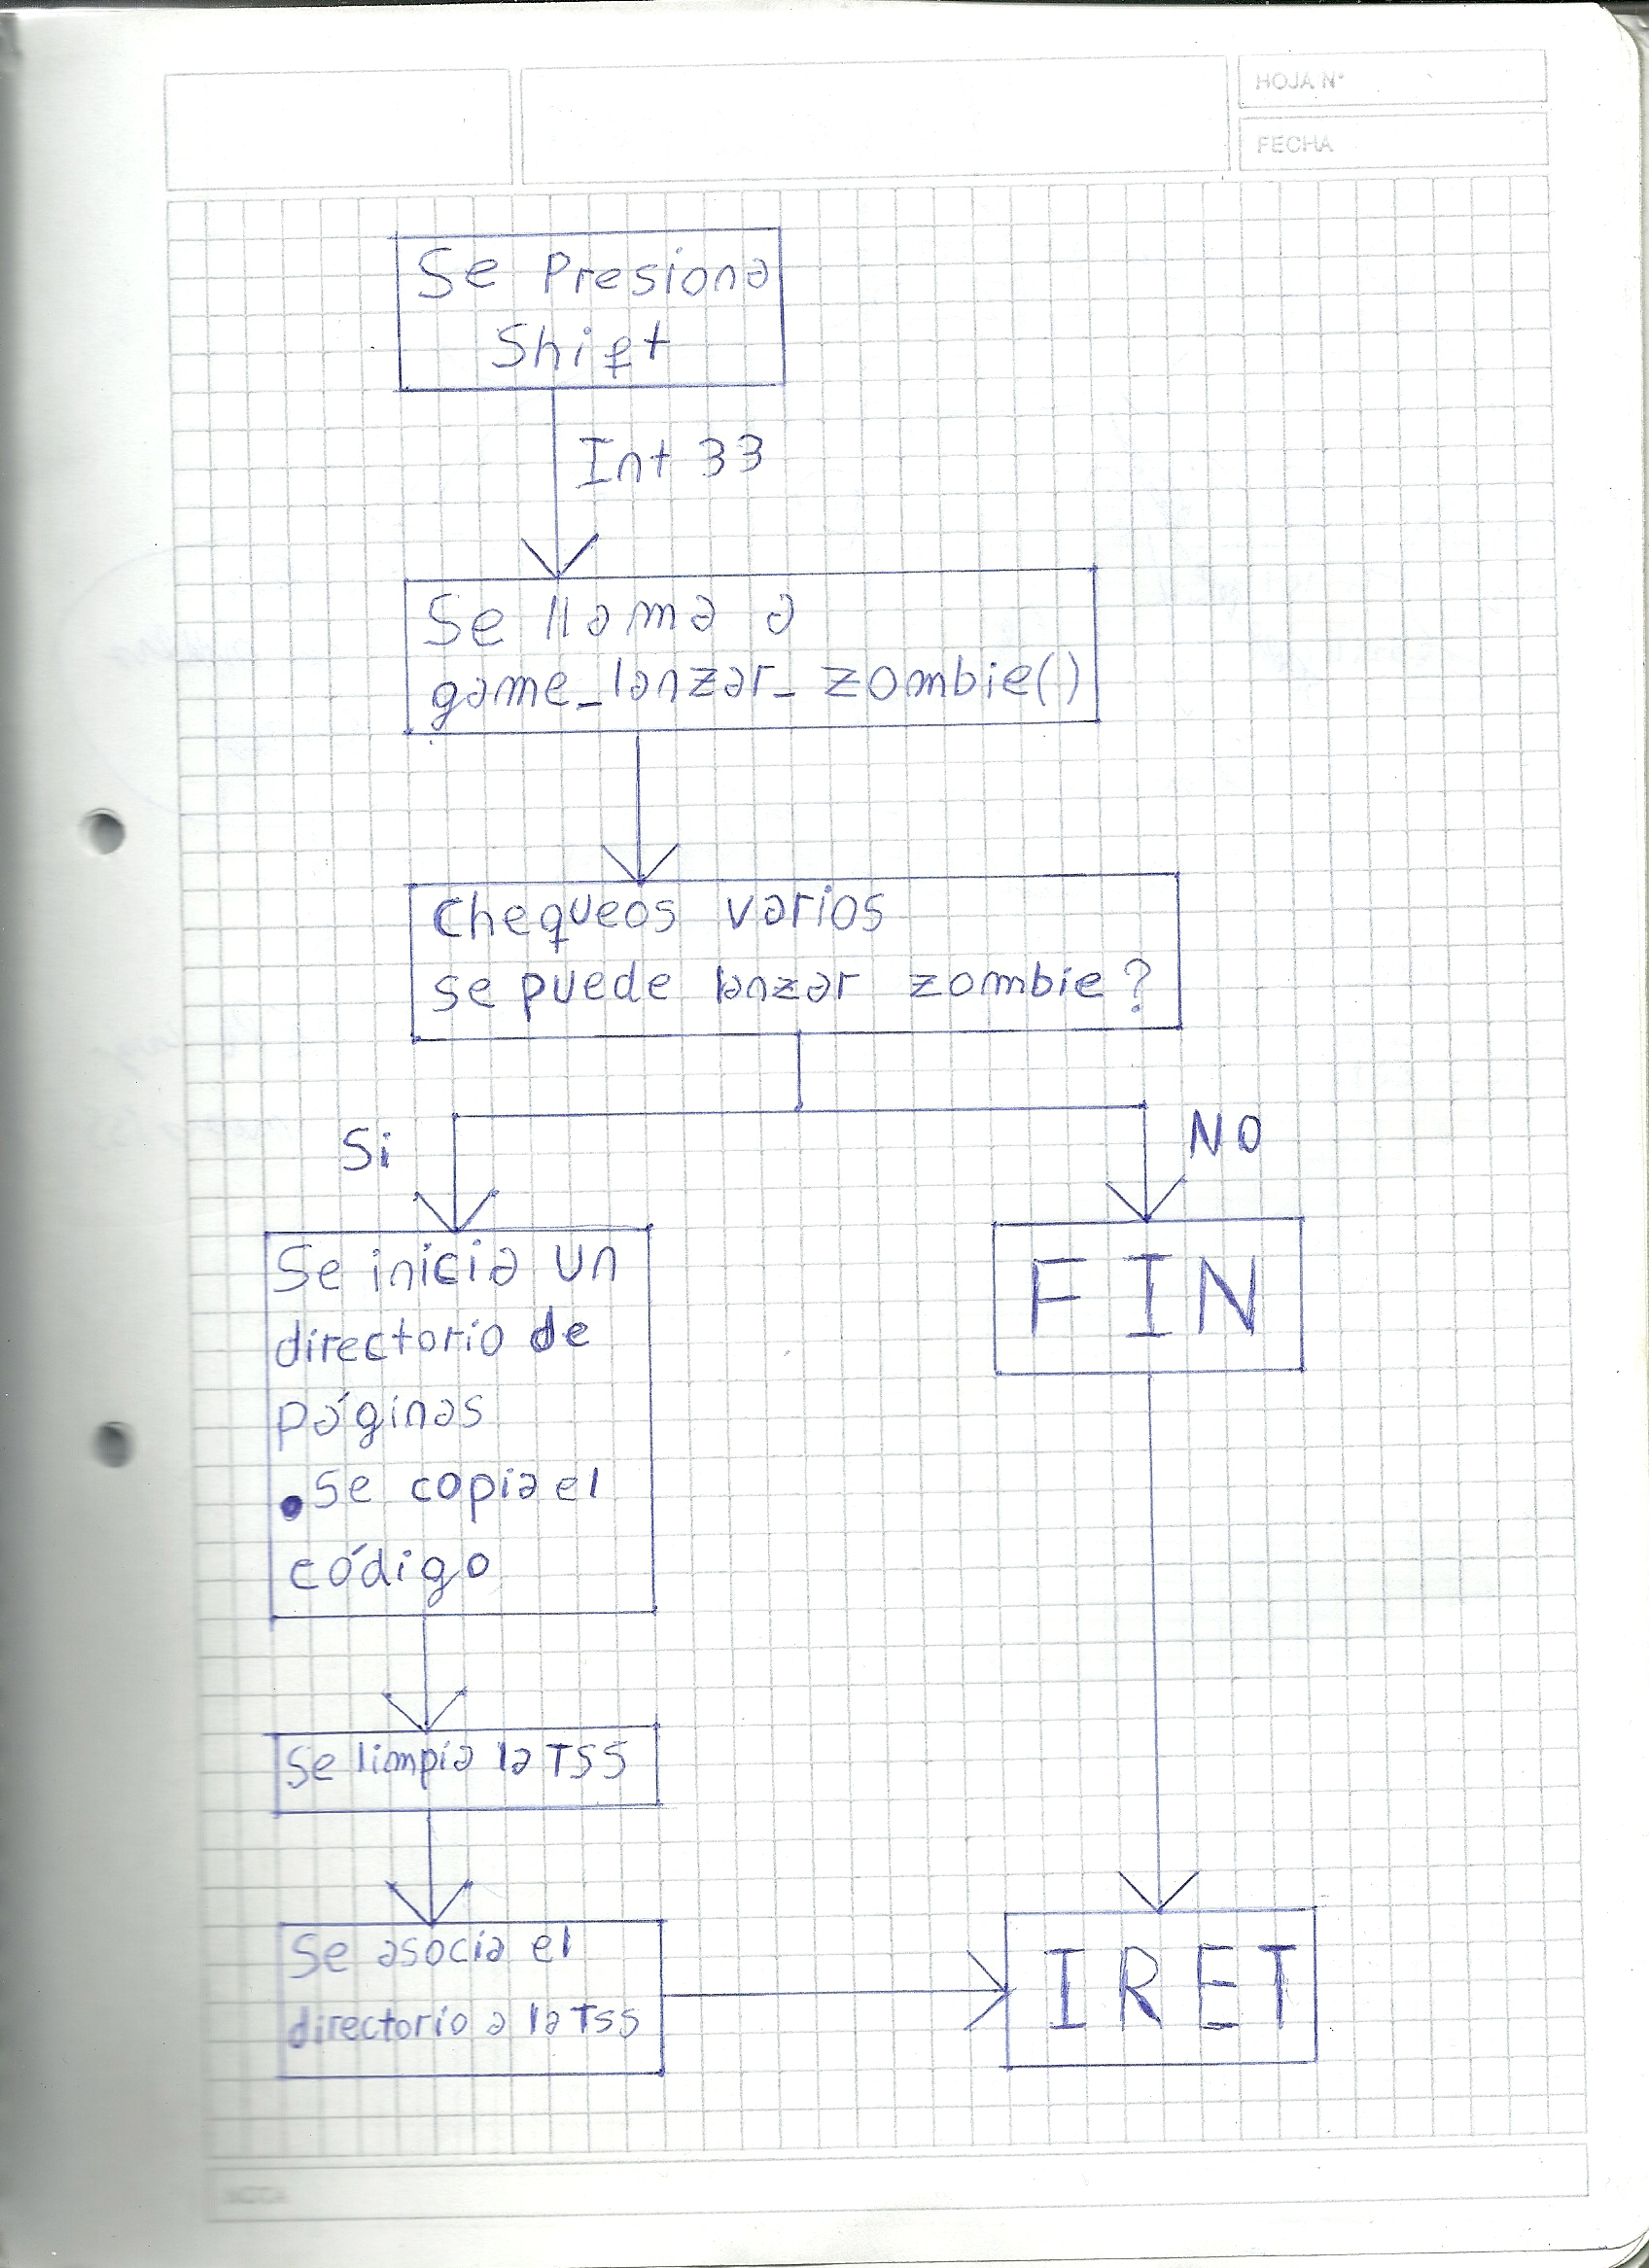
\includegraphics[scale=0.2]{dibujos/dibujo1.jpg}\\
%  \end{center}
%\end{figure}
\newpage

Notamos además que este arreglo de si los zombies están muertos o vivos puede resultar muy útil para indicarle al scheduler cuál tarea correr, así que se reimplementa el scheduler para que le pregunte a través de $game\_ proximo\_ zombie()$ cuál será el proximo zombie a ejecutar.

Para encapsular todo el comportamiento de escribir en el bufer de video y hacer mas claro el codigo se implementa todo el comportamiento de escribir en la pantalla en $game\_actualizarFrame()$. Dado que como hemos dicho, en $game.c$ esta guardado todo la informacion de jugadores y zombies, cada vez que la función es llamada, se refresca la pantalla por completo, rescribiendo tanto zombies como puntajes, posiciones de los jugaores, etc.

Dada que esta función se debe ejecutar de manera periodica, se decide llamar a esta función desde la int $32$ para que con cada tic de clock del procesador se actualice la pantalla, aunque el framrate sería facilmente ajustable haciendo que en vez de llamarse con cada tic se llame cada $2, 4$ o lo que se decida.(Nota: nuestro juego corre a mas de 60 FPS, TAKE THAT PS4).

En el siguiente esquema se muestra de manera general como funcionará la int $32$:


%\begin{figure}[h!]
%  \begin{center}
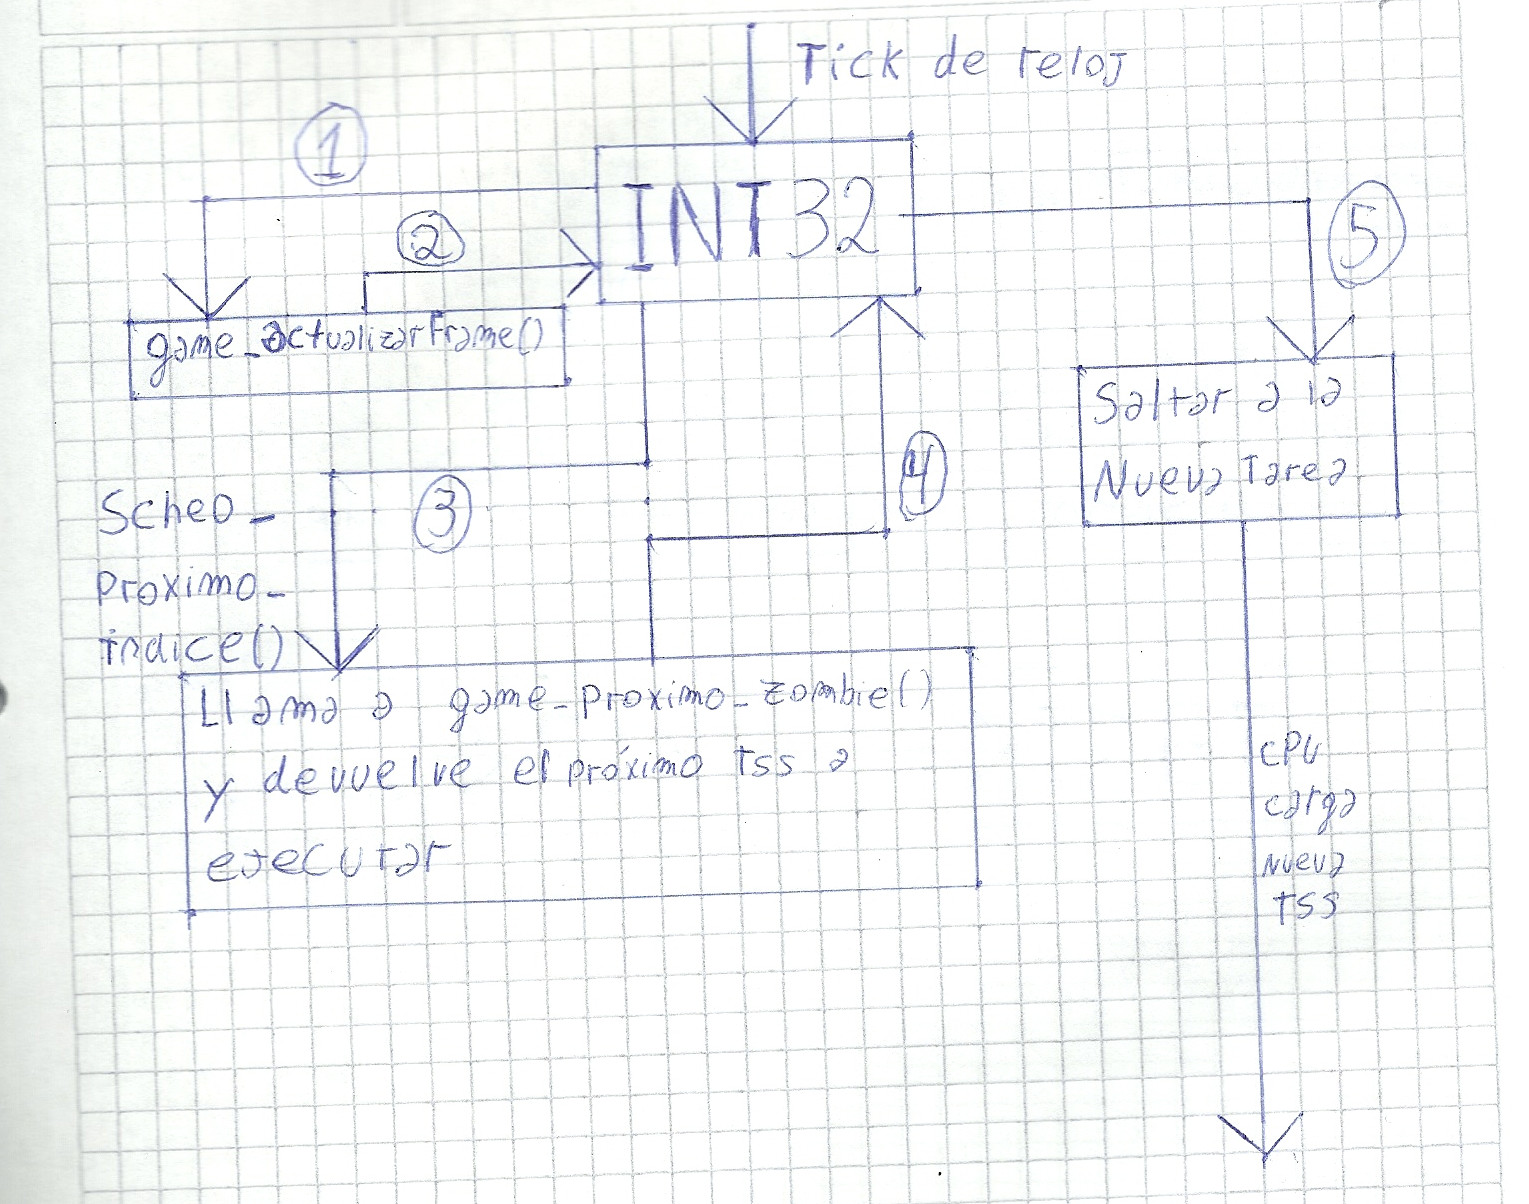
\includegraphics[scale=0.9]{dibujos/dibujo2.jpg}\\
%  \end{center}
%\end{figure}
\newpage


Llegados a este punto ya es posible lanzar zombies al campo de juego, intercambiar sus tareas para que corran concurrentemente y ejecutarlos debidamente. Por supuesto, como la int $0x66$ todavía no tiene ninguna funcionalidad, el zombie permanece en su lugar.

Se procede a implementar esta funcionalidad en $game_move\_current\_zombi()$ . Se decide que la mejor manera de realizar esto es, que para mover un zombie, primero se muevan las coordenadas en X e Y del mismo hacia la direccion que correspona, luego, con una función apropiada, se determine para esa pocición y dependiendo de si es el jugador A o B, cual será el mapeo pertinente y se llame a una función $mmu\_remapearPaginasZombie()$ que tome las direcicones calculadas previamente y las remapee segun corresponda en el cr3 actual (El CR3 actual siempre es el del zombie que pidió la interrupción).

Ademas, se aprovecha $game\_move\_current_zombi()$ para que chequee las pociciones de X e Y para saber si el zombie esta en una posición valida y se anote un punto si llegó al otro lado del tablero.

El esquema de este funcionamiento es:


%\begin{figure}[h!]
%  \begin{center}
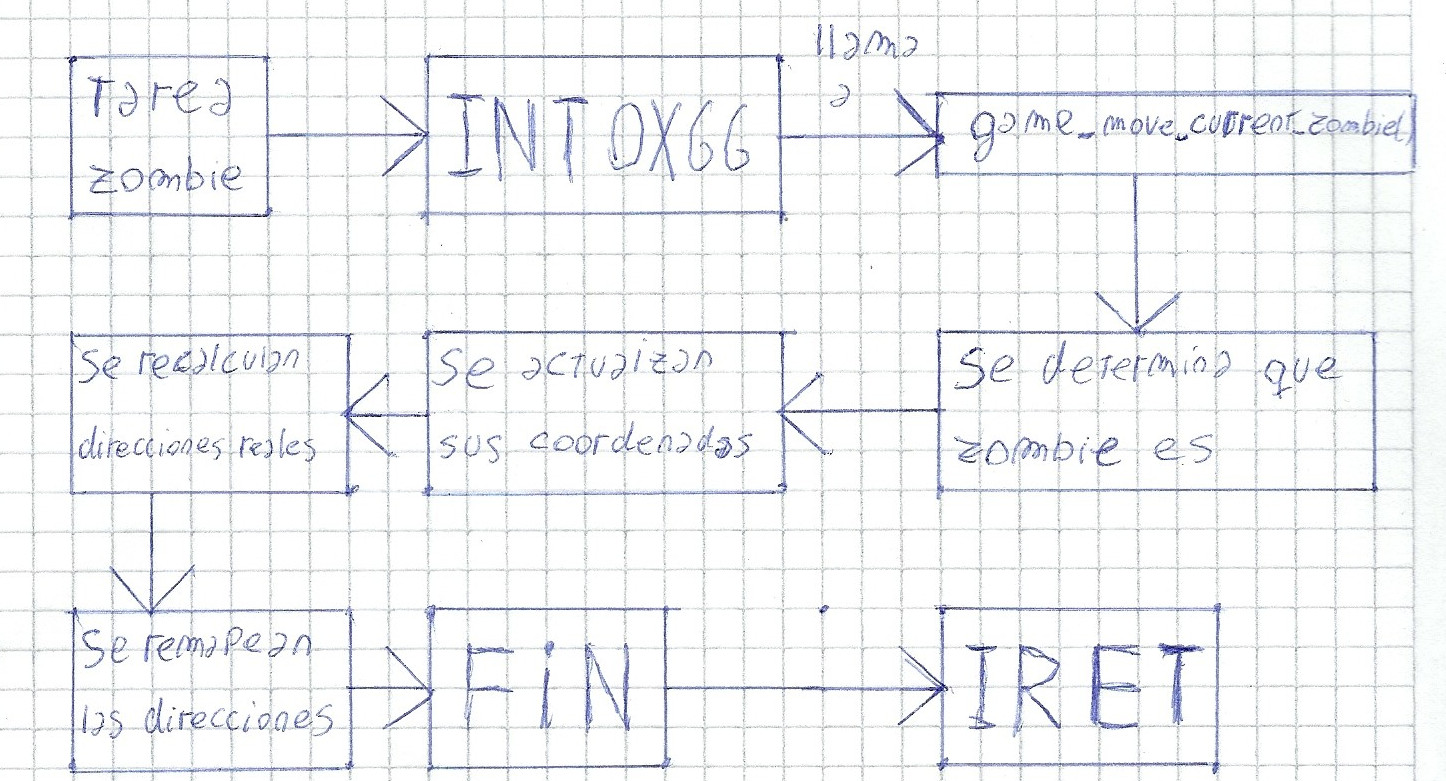
\includegraphics[scale=0.9]{dibujos/dibujo3.jpg}\\
%  \end{center}
%\end{figure}
\newpage

Muy bien, ya casi terminamos!. Ahora vemos como los zombies corren libres por el tablero de juego, cada uno con sus correspondientes paginas siendo remapeadas cada vez que llaman a la int $0x66$. Sin embargo el zombie mago entregado por la catedra, produce una general protection que al no ser manejada de la manera debida, detiene el juego.

Se decide implementar en C una nueva función que será llamada por todas las interrupciónes $game\_error\_handling()$ la misma buscará que TSS causó la interrupción. A partir de eso, es trivial determinar que jugador y que zombie causaron ínterrupción. Luego, para ese zombie en particular se setea su ya mencionado $clockZombie$ en "muerto". De esa manera $game\_ proximo\_ zombie()$ no tomará a ese zombie como candidato y el scheduler no volverá a ejecutar esa TSS salvo que otro zombie se inicialice en ese espacio determiando. (Nota: En principio se intentó limpiar la TSS en este momento, pero limpiar la TSS de una tarea activa resultó ser una mala idea.)

Luego de ser manejada la interrupción se vuelve a saltar a la tarea idle y se continúa con la ejecución normal.

Solo queda implementar el modo debug, para eso simplemente se decide implementar una interrupción de teclado para la tecla Y que ponga una dword en 1 en caso de que sea precionada. Luego, al llamarse a una interrupción, se llama a una función en C que imprime todo lo necesario por pantalla y luego se queda haciendo pooling del teclado hasta que la tecla Y sea precionada nuevamente.

\end{document}

